\documentclass[12pt,onecolumn]{report}

\usepackage[pdftex]{graphicx}
%\usepackage[footnotesize]{caption}
%\usepackage[footnotesize]{subfigure}
\usepackage{textcomp}
\usepackage[usenames, dvipsnames]{color}
\usepackage{amsmath,amsfonts,amsthm,amssymb}
\usepackage{setspace}
\usepackage{Tabbing}
\usepackage{fancyhdr}
\usepackage{lastpage}
\usepackage{graphics}
\usepackage{comment}
\usepackage[T1]{fontenc}
\usepackage{mdwlist}
\usepackage[cmyk]{xcolor}
\usepackage{bibentry}


% Adjust margins:
%\topmargin=-0.45in      %
%\evensidemargin=0in     %
%\oddsidemargin=0in      %
%\textwidth=6.5in        %
%\textheight=9.0in       %
%\headsep=0.25in         %
\usepackage[margin=1.00in]{geometry}
\usepackage{setspace}
\doublespacing

%\newcommand{\Section}[1]{\section{#1} \setcounter{figure}{1}}
\renewcommand\thesection{\arabic{section}}


% Homework Specific Information
\newcommand{\hmwkTitle}{Manipulator Research and Assembly}
\newcommand{\hmwkDueDate}{}
\newcommand{\hmwkClass}{Multi-Robot Systems Lab}
\newcommand{\hmwkClassInstructor}{Dr. James McLurkin}
\newcommand{\hmwkAuthorName}{Amanda Boone, Kevin Koch}


% Header and Footer:
\headheight = 15pt
\pagestyle{fancy}
\lhead{Boone, Koch}
\chead{}
\rhead{\hmwkClass\ : \hmwkTitle}
\lfoot{} 
\cfoot{}
\rfoot{Page\ \thepage\ of\ \pageref{LastPage}} 
\renewcommand\headrulewidth{0.4pt}
\renewcommand\footrulewidth{0.4pt}


% Title:/
\title{\textmd{\Huge{\textbf{\hmwkTitle}}}\\
\Large{\textbf{\hmwkClass:\ \textit{\hmwkClassInstructor}}}\vspace{0.75in}
}
%
\vspace{1in}
\author{\Large{\textbf{\hmwkAuthorName}}}

\begin{document}
\maketitle
%\tableofcontents
%\addtocontents{toc}{\protect\thispagestyle{fancy}}

%change 0.1 to 1 for numbering purposes.
\renewcommand*\thesection{\arabic{section}} 

\newpage
\onehalfspacing

\begin{figure}[ht]
\begin{center}
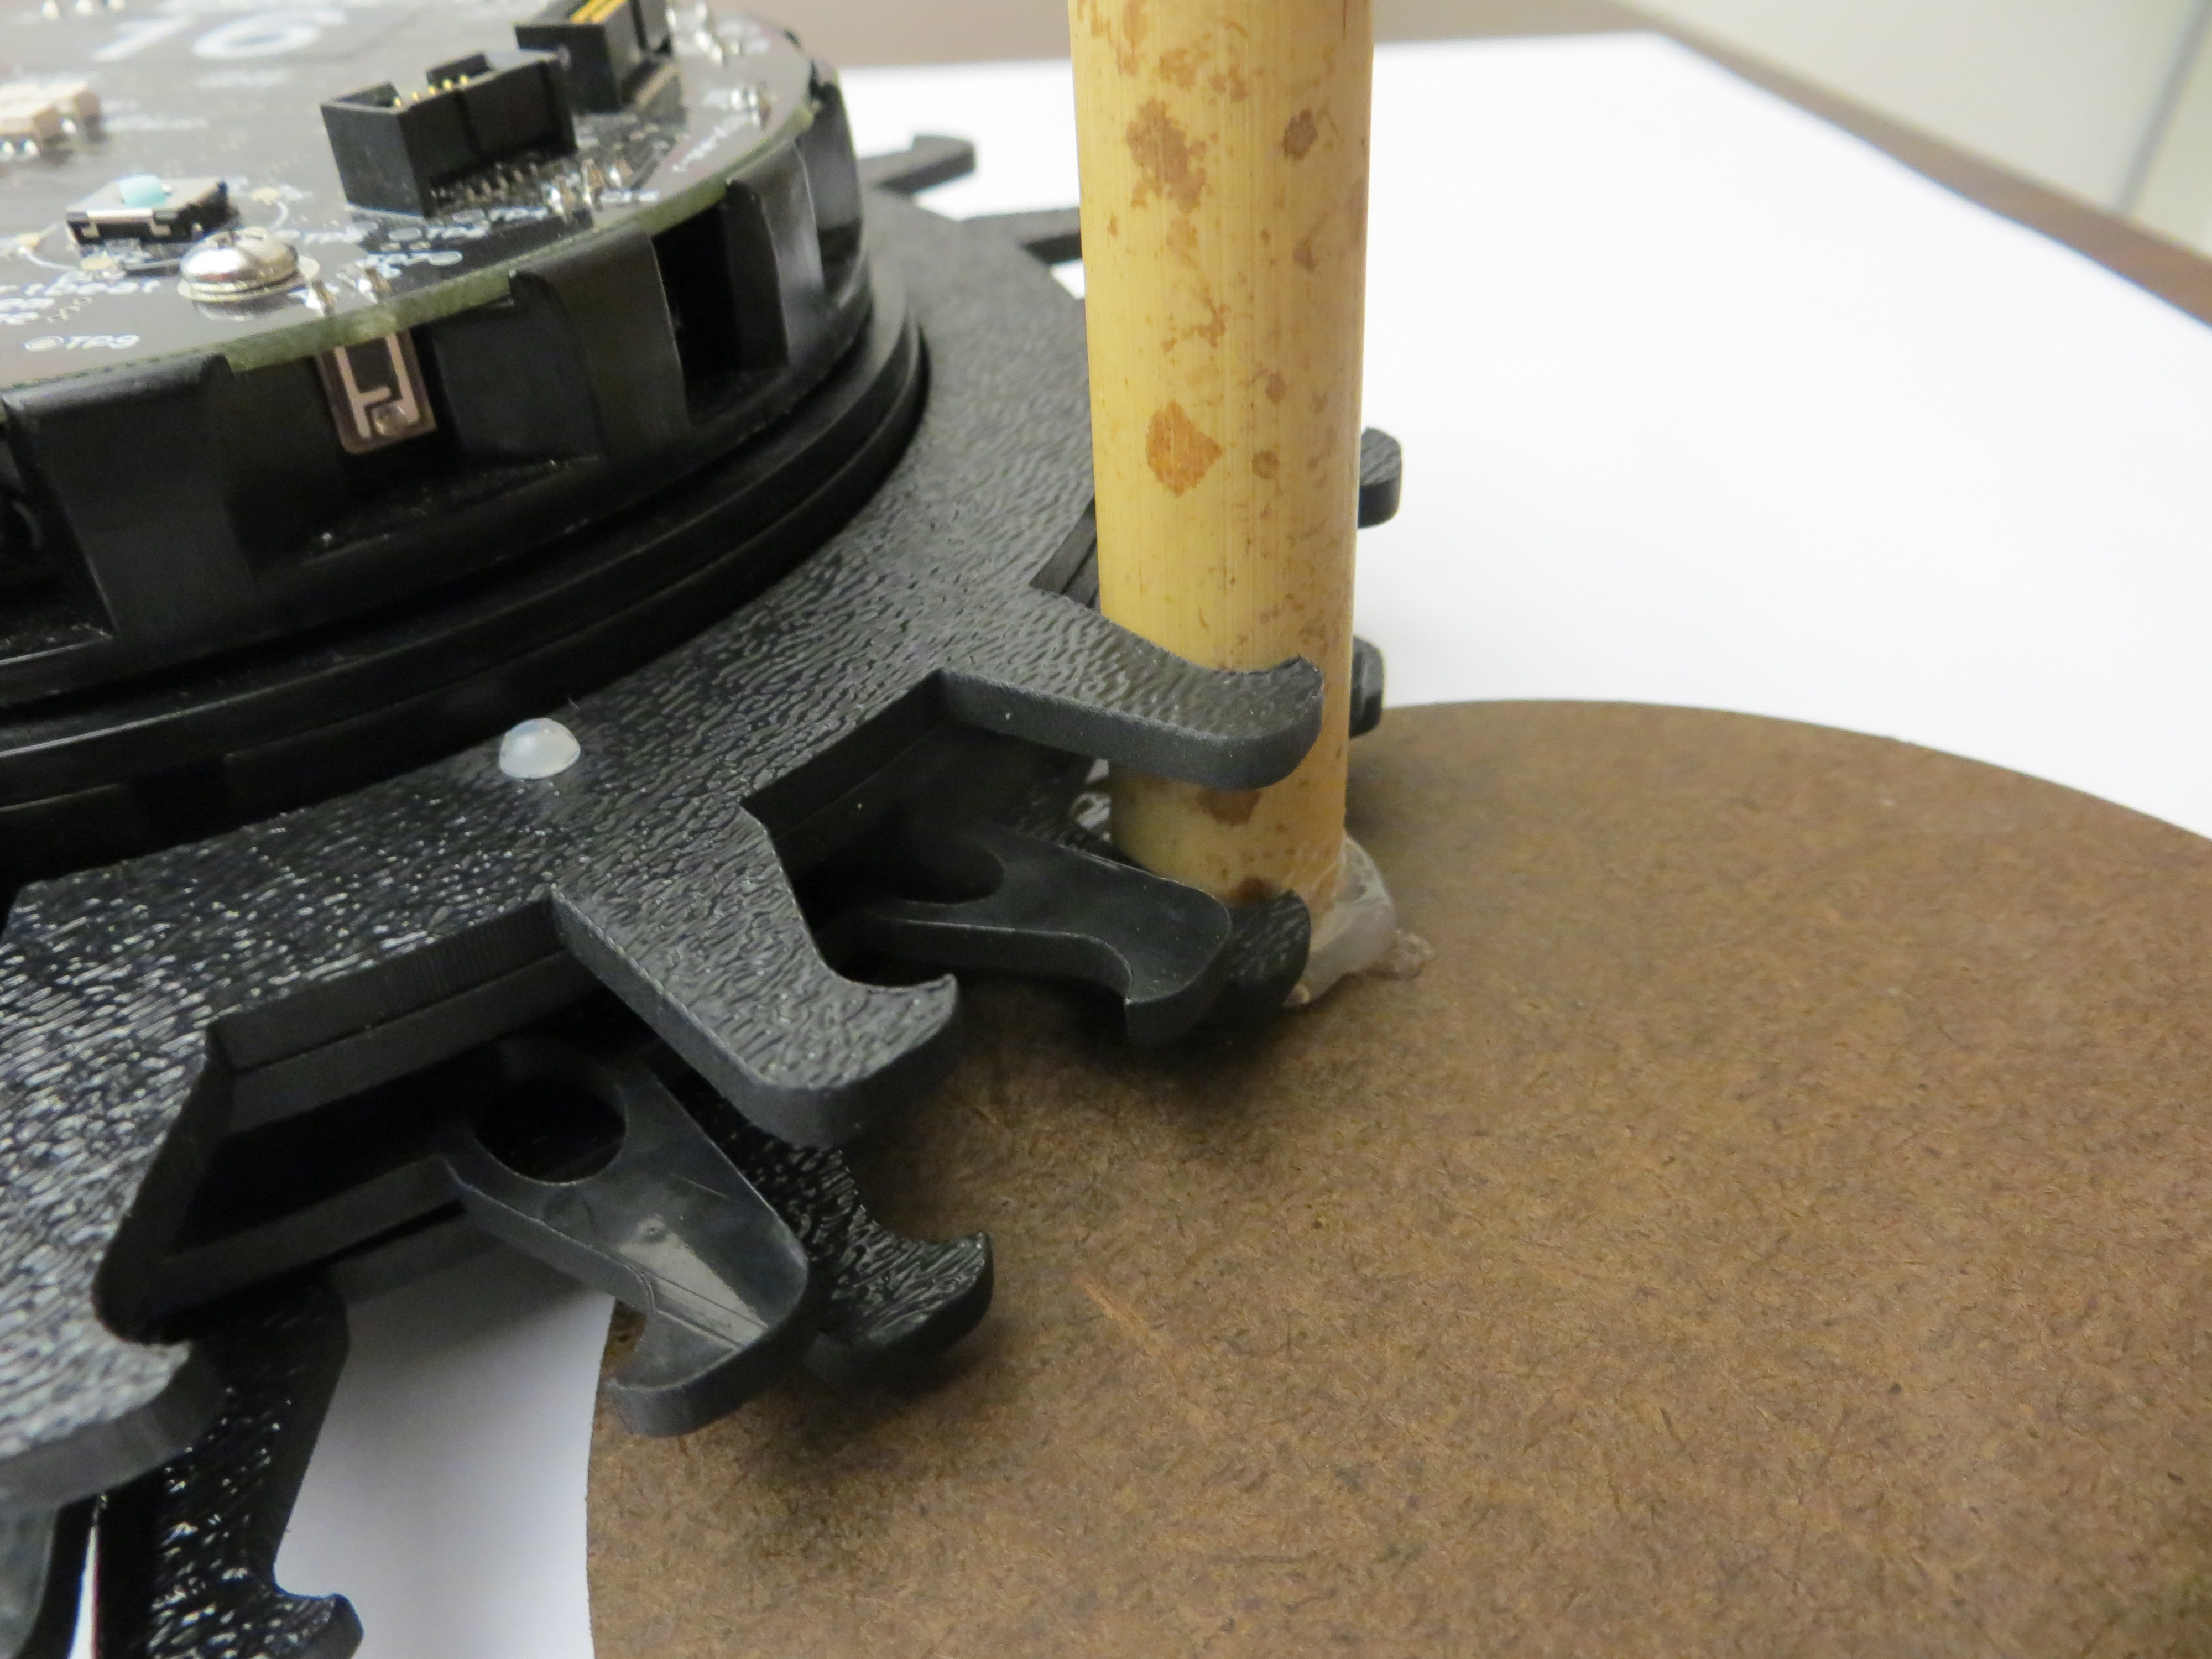
\includegraphics[width=.5\linewidth]{./Figs/close_grab.jpg}
\end{center}
\caption{This is a close-up view of the robot so, showing that we chose a three claw design so that there would be no pinching or twisting of the object or of the manipulator.}
\label{fig:Grab}
\end{figure}

After initially sitting down at the drawing board, Amanda and I went through many iterations of design options with this prototype actuated manipulator. 
We decided on the servo-actuated gripper because of its relatively simple design, functionality, and expandability. We decided to use three claw levels with only one actuated claw disk because it provides the best stability of the item that it is grabbing. The three claws provide three points of contact with the item, such as a pen, and thus hold the item more straight up and down than if we were to use a two claw design that would pinch and twist the item, shown in Figure \ref{fig:Grab}. ABS plastic was chosen because of both its strength and lightweight properties. It is stronger than wood, and this is beneficial because the servo exerts a good amount of torque, which would cause the small pieces of wood to break. An added bonus of the ABS that we chose was that it has a very low coefficient of friction on the textured side, which is great for the movement of the pieces.
We decided against more complex designs such as an inverted gear or rotary linkage for the initial prototype due to time constraints and simplicity. Keeping things as simple as possible has always worked out the best for us, so that's what we chose. 

\begin{figure}[ht]
\begin{center}
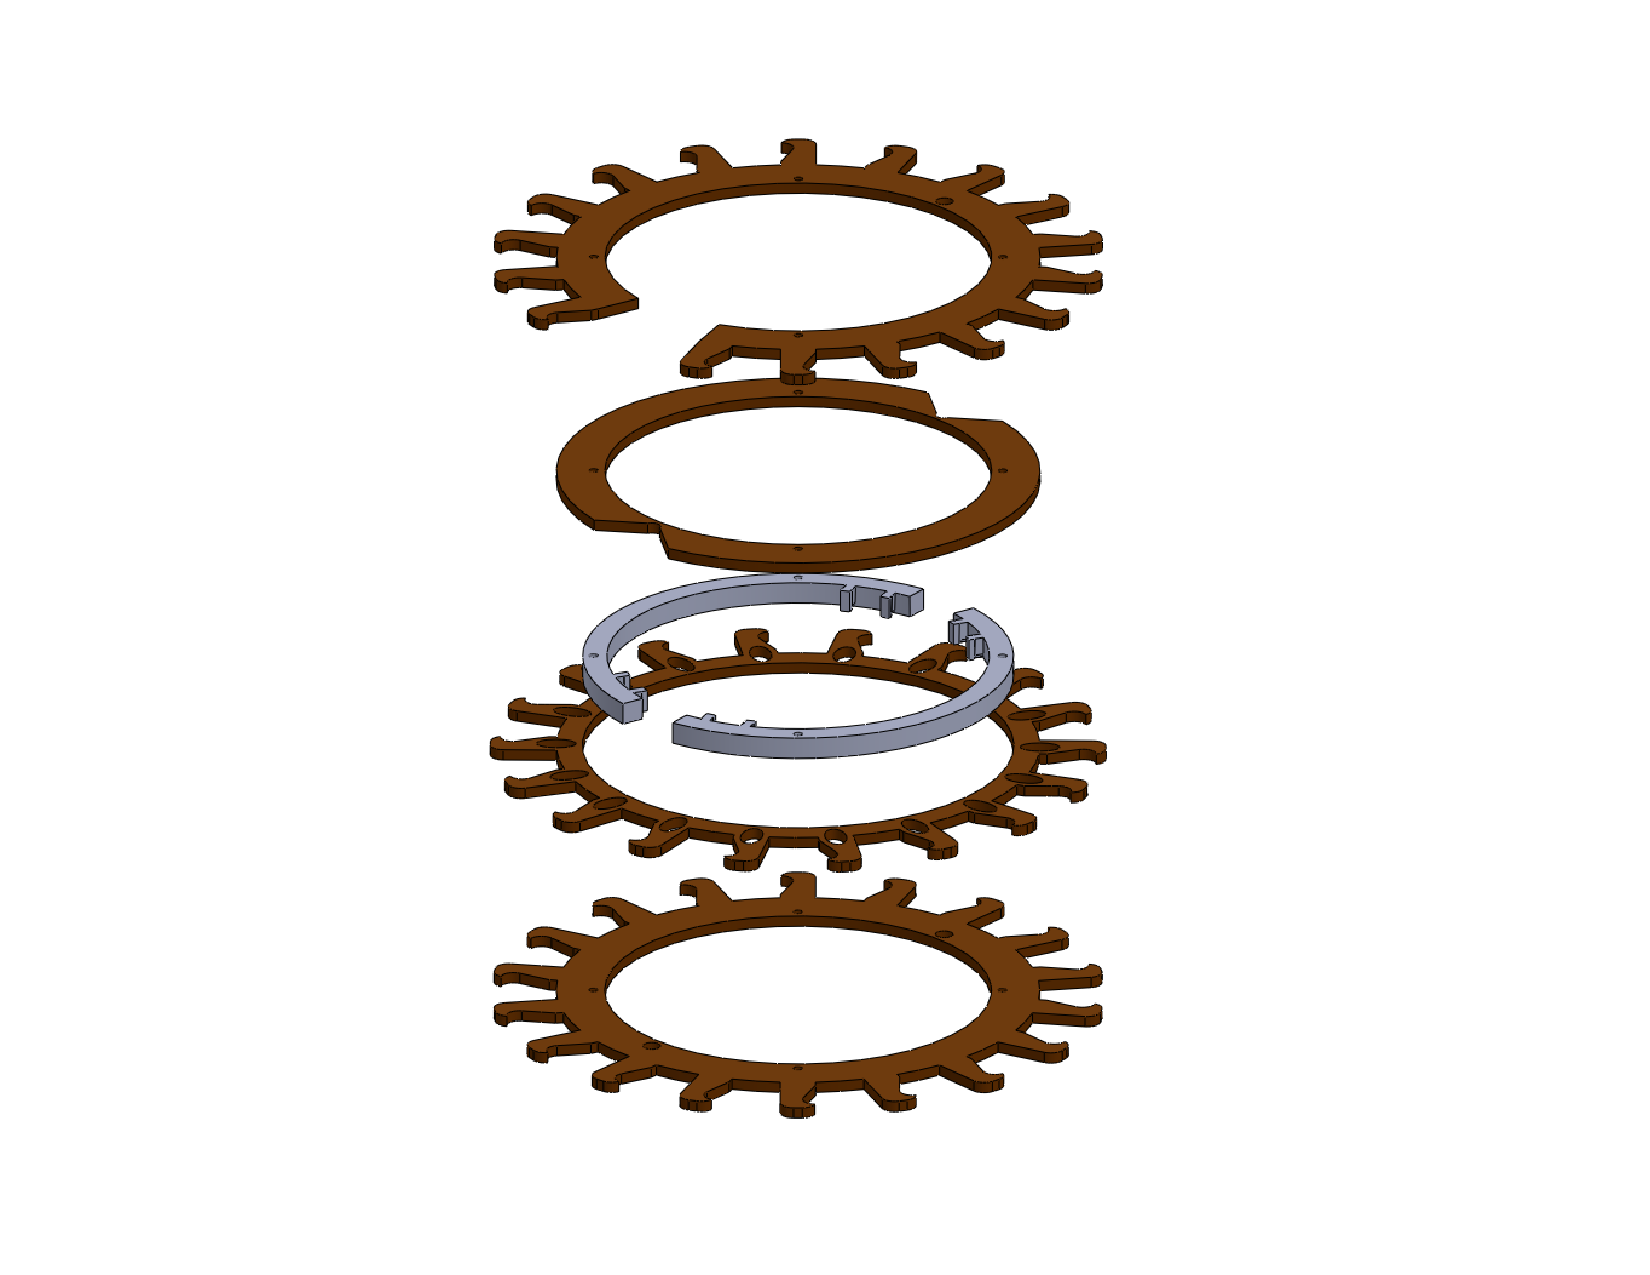
\includegraphics[width=.5\linewidth]{./Figs/final_assembly_explodedisometric.pdf}
\end{center}
\caption{An exploded view of the CAD model of the Actuated Manipulator}
\label{fig:explode}
\end{figure}

\begin{figure}[ht]
\begin{minipage}[b]{0.45\linewidth}
\centering
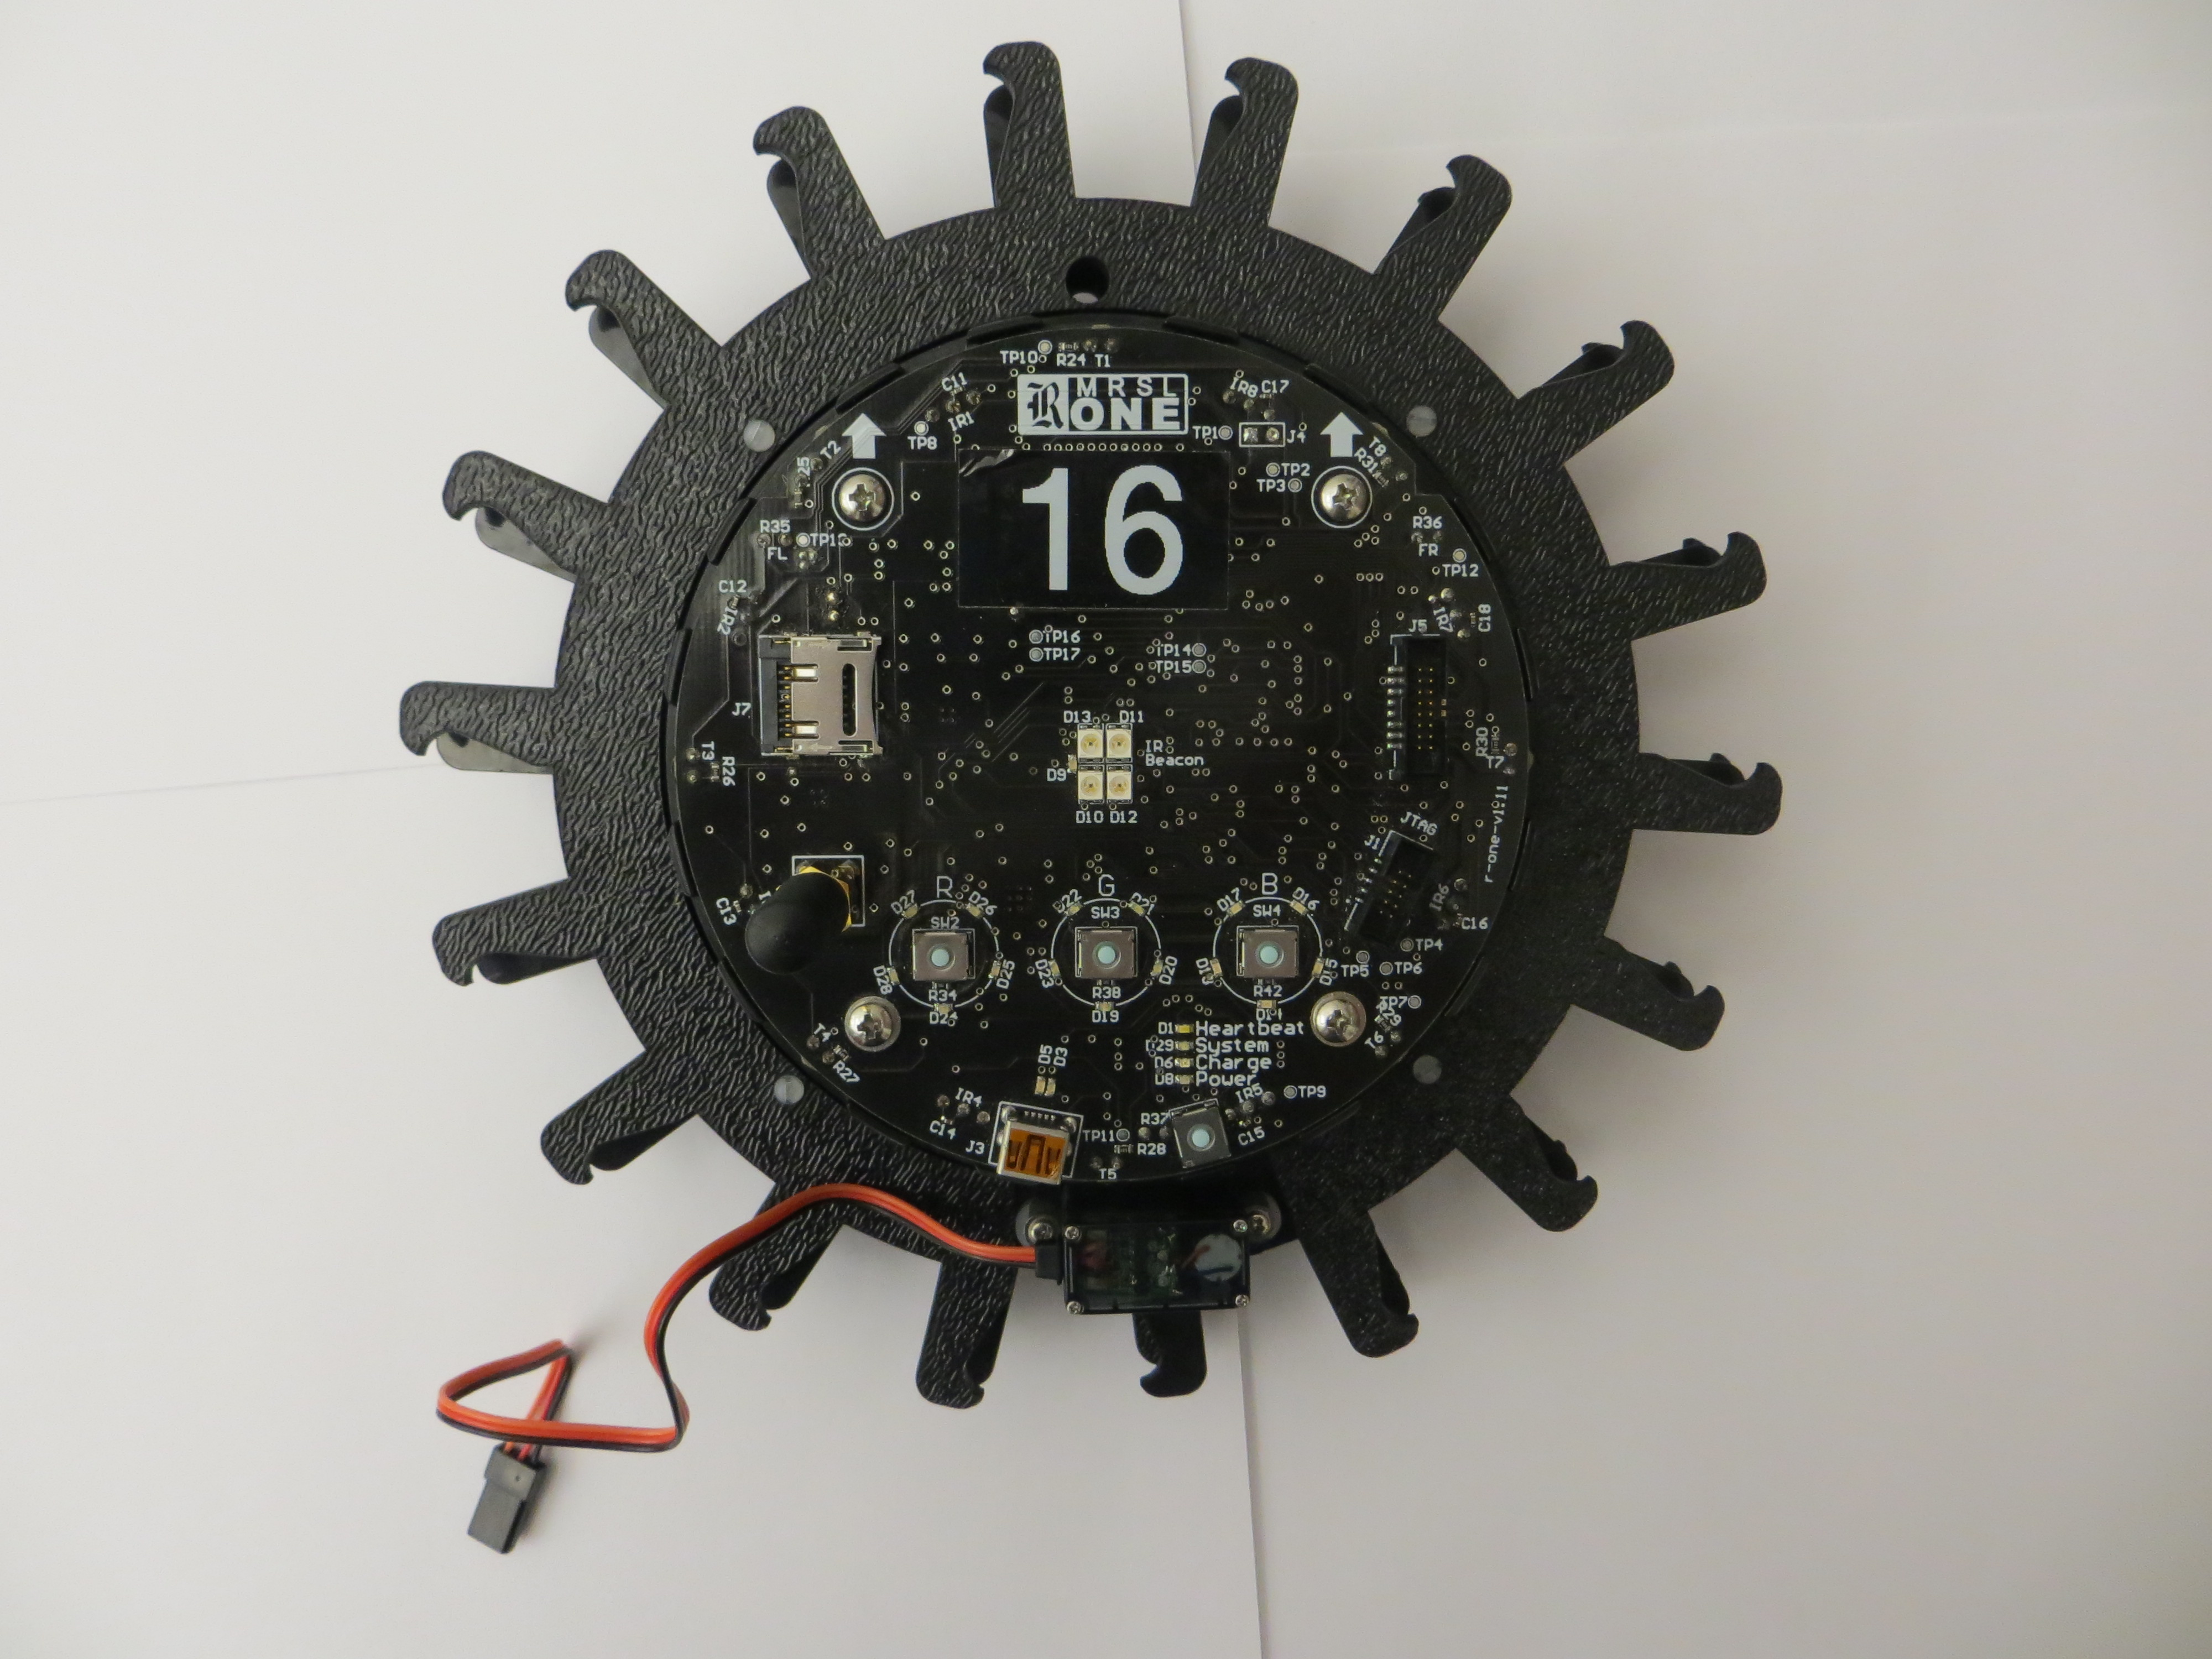
\includegraphics[width=.45\linewidth]{./Figs/top_closed.jpg}
\caption{A top view of the robot with the manipulator fully closed}
\label{fig:closed}
\end{minipage}
\hspace{0.5cm}
\begin{minipage}[b]{0.45\linewidth}
\centering
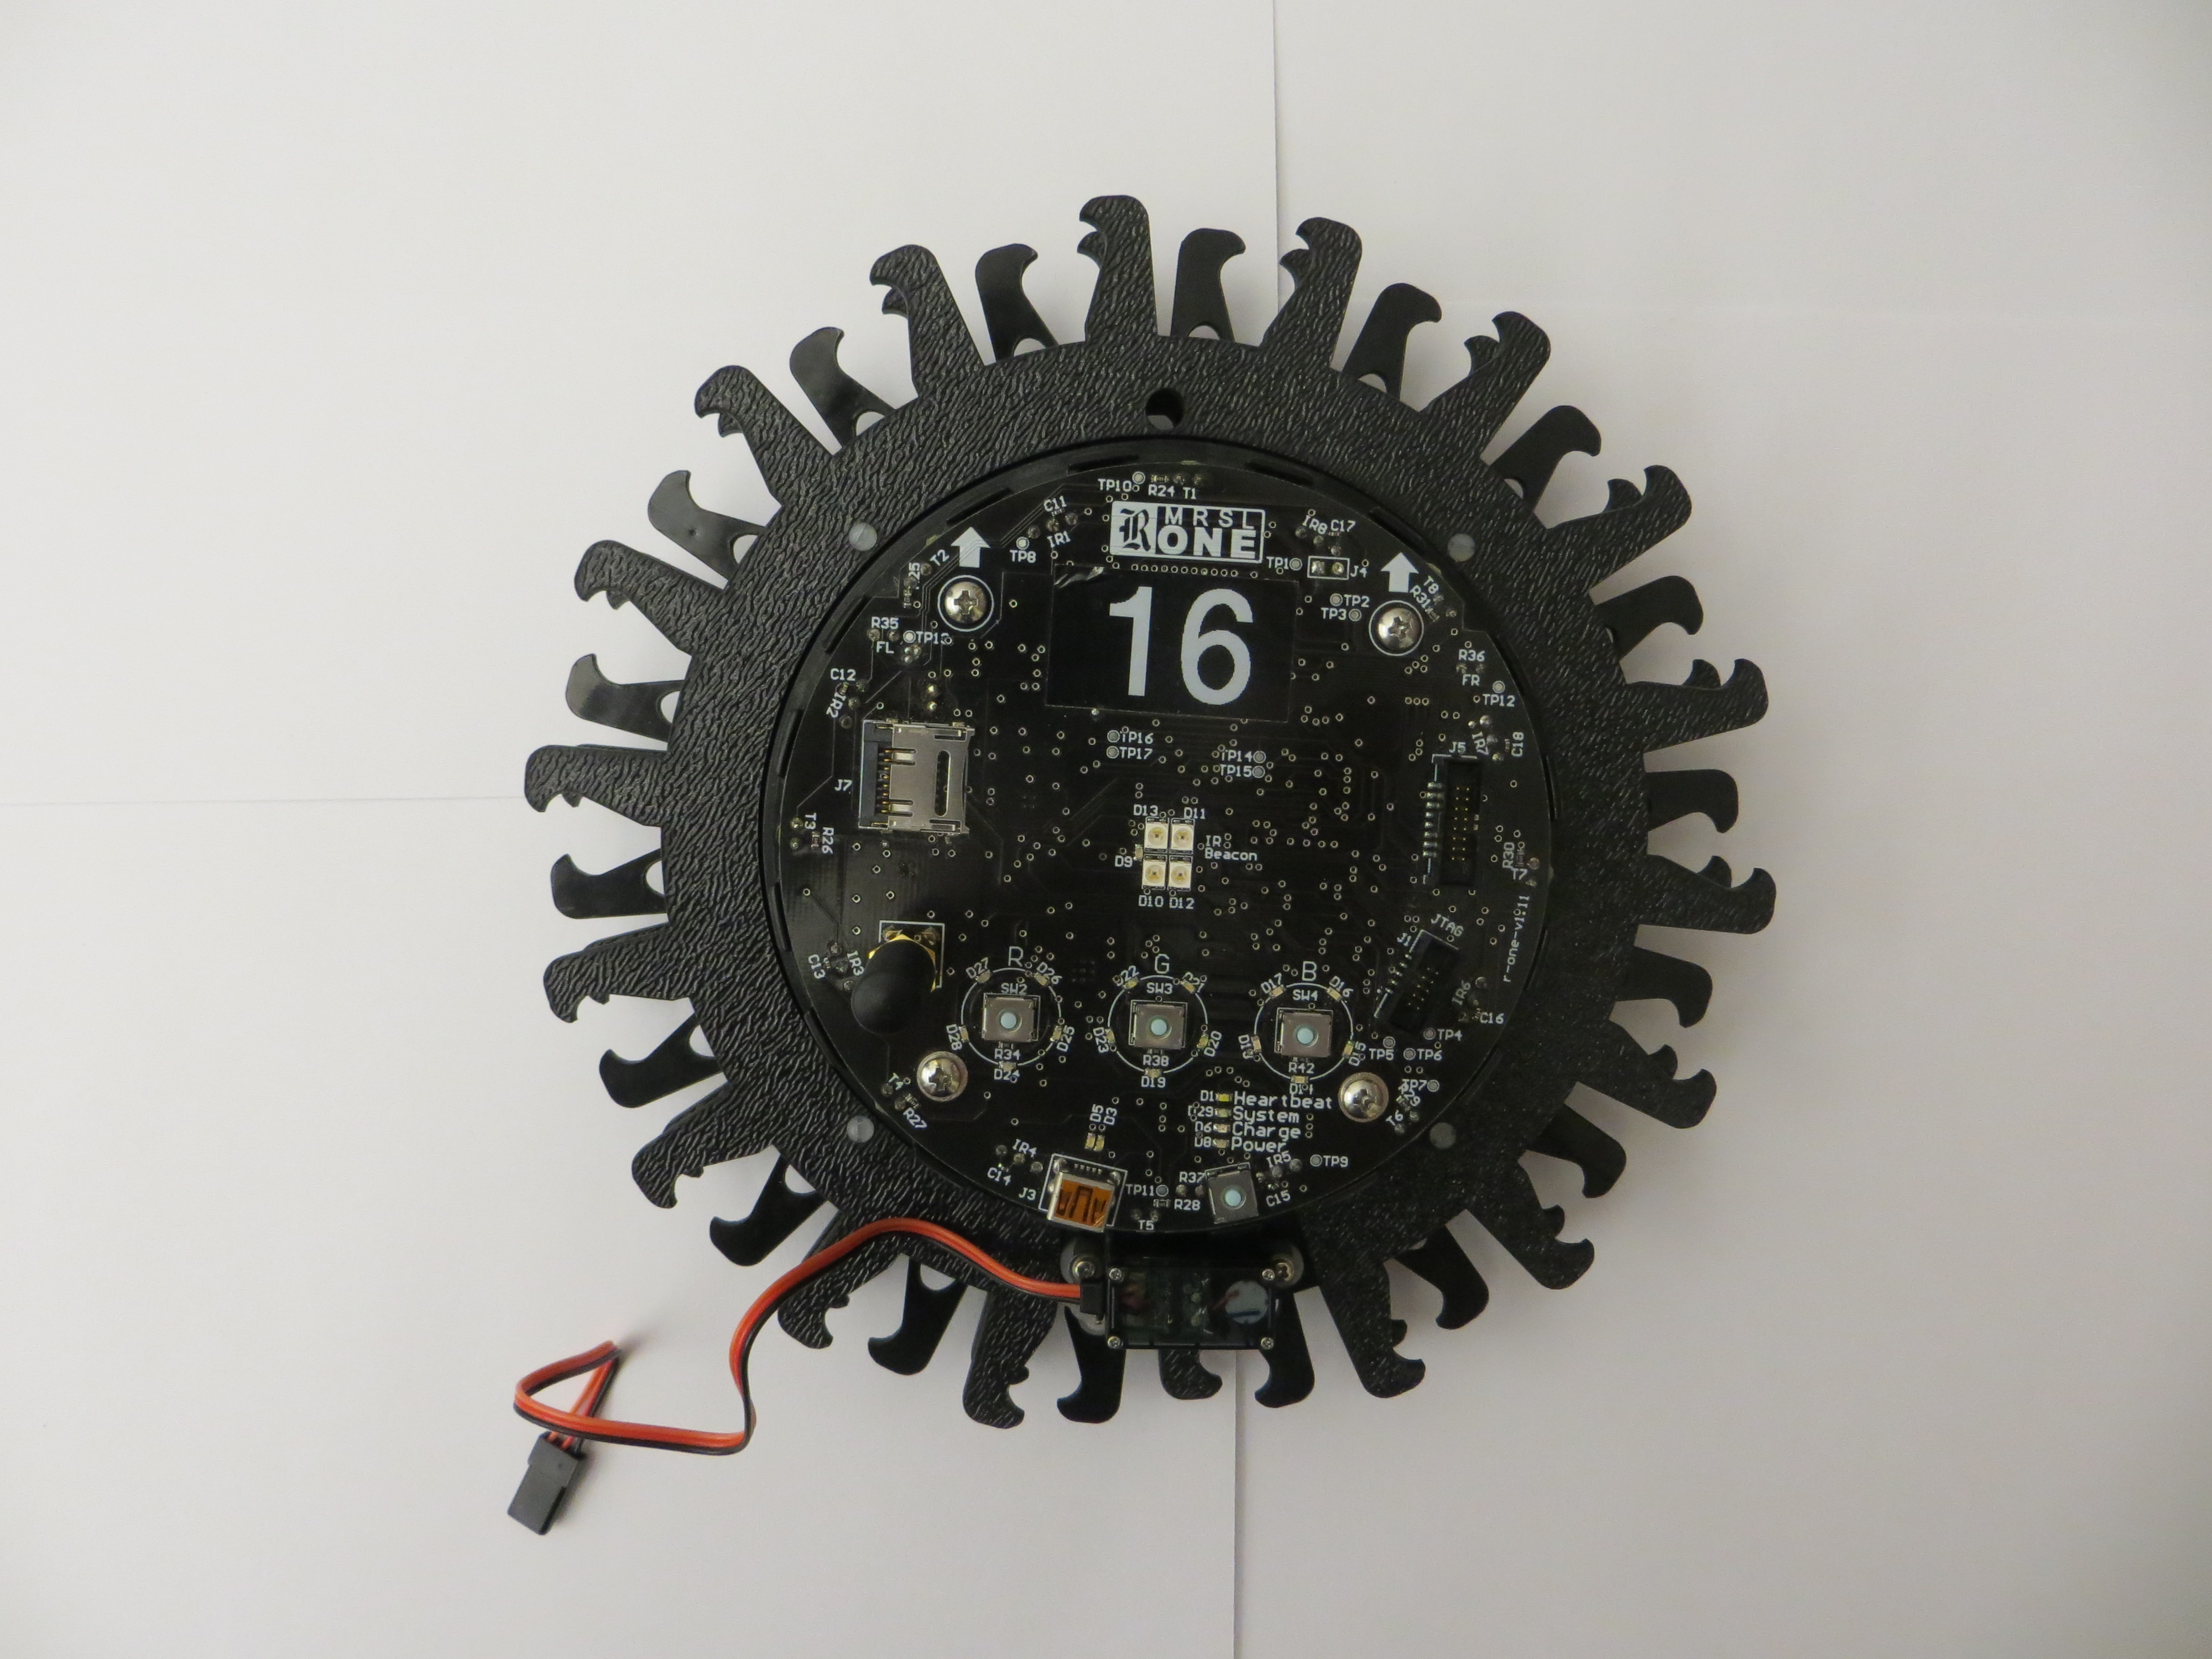
\includegraphics[width=0.45\linewidth]{./Figs/top_open.jpg}
\caption{A top view of the robot with the manipulator fully open.}
\label{fig:open}
\end{minipage}
\end{figure}

Our prototype uses the same clips as the Velcro Manipulator, however, they are just cut the ends to allow for the turning of the servo arm. The claws are made this way because we want the robots to be able to grab other robots as well as the objects made for the robot world, smooth manipulators would grab nothing. 

There are a few issues with our current prototype that have to be addressed, however we ran out of time to fix them, but we have analyzed and diagnosed them. The first of which is the current peg on the robot that is attached to the servo must be fixed. It rubs and catches on the very bottom claw disk and prevents full motion, as can be seen in the video and in Figure \ref{fig:problem}. Next to be revamped, the slots used to rotate the manipulator, they are too big and allow for too much play in the rotation, posing slight issues unless we used large spacers like the ones we did. This can be fixed through the use of a smaller slit and a simple pin going down from the servo arm. The next issue we did not have time for was the counter-rotation issue. We propose that, in order to get free rotation of the manipulator around the robot, we must counter-rotate the manipulator claws, so that there is still torque applied to an object regardless of which way the robot spins. Power transmission is the other issue with this, contact strips along the outside of the robot, onto which contacts to the servos rub in order to get power seems like the simplest option, albeit fairly complex.

\begin{figure}[ht]
\begin{center}
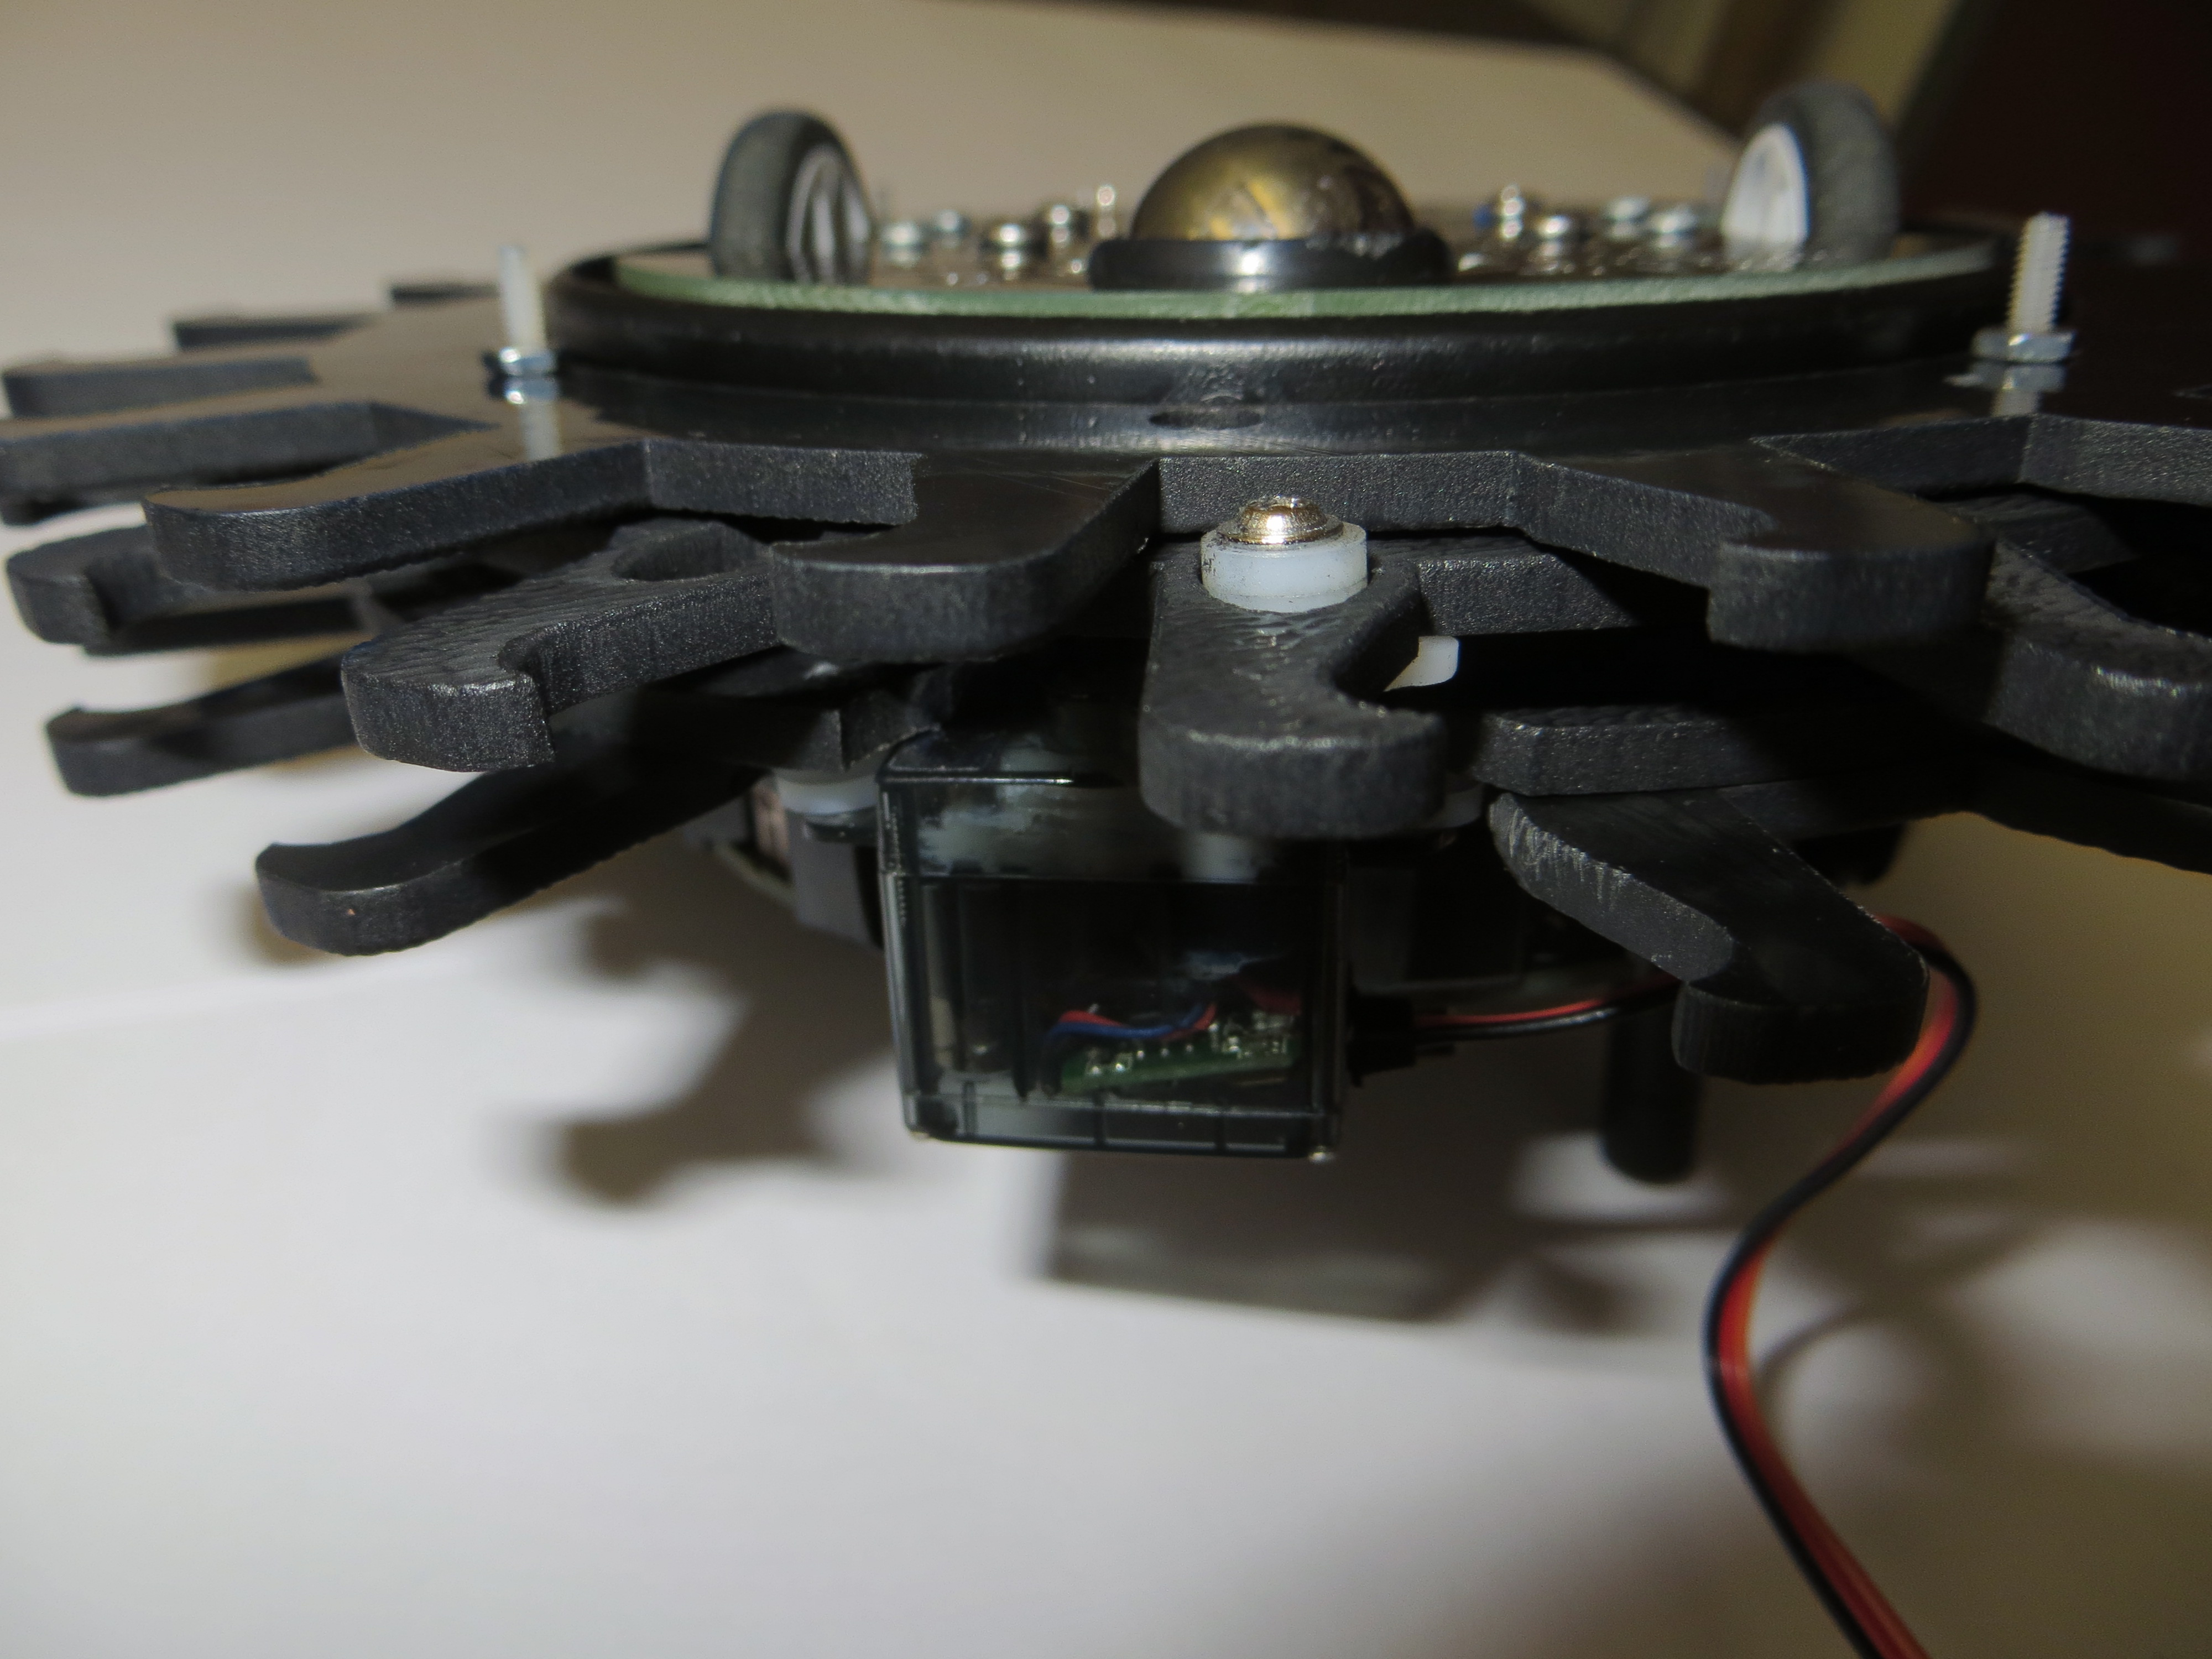
\includegraphics[width=.5\linewidth]{./Figs/bottom_problem.jpg}
\end{center}
\caption{This is currently the worst issue we face, the pin extrudes into the plane of the bottom claw disk, causing it to catch and prevent movement.}
\label{fig:problem}
\end{figure}

We did research in order to determine the most accurate way to detect whether the robot had indeed grabbed something or not, and this was to analyze the current change with different forces acting on the servo. We did this by hanging weights on a lone servo acting at 35.75 mm moment arm and comparing that to the servo that actuates the manipulator, again, by hanging weights. 

\begin{figure}[ht]
\begin{center}
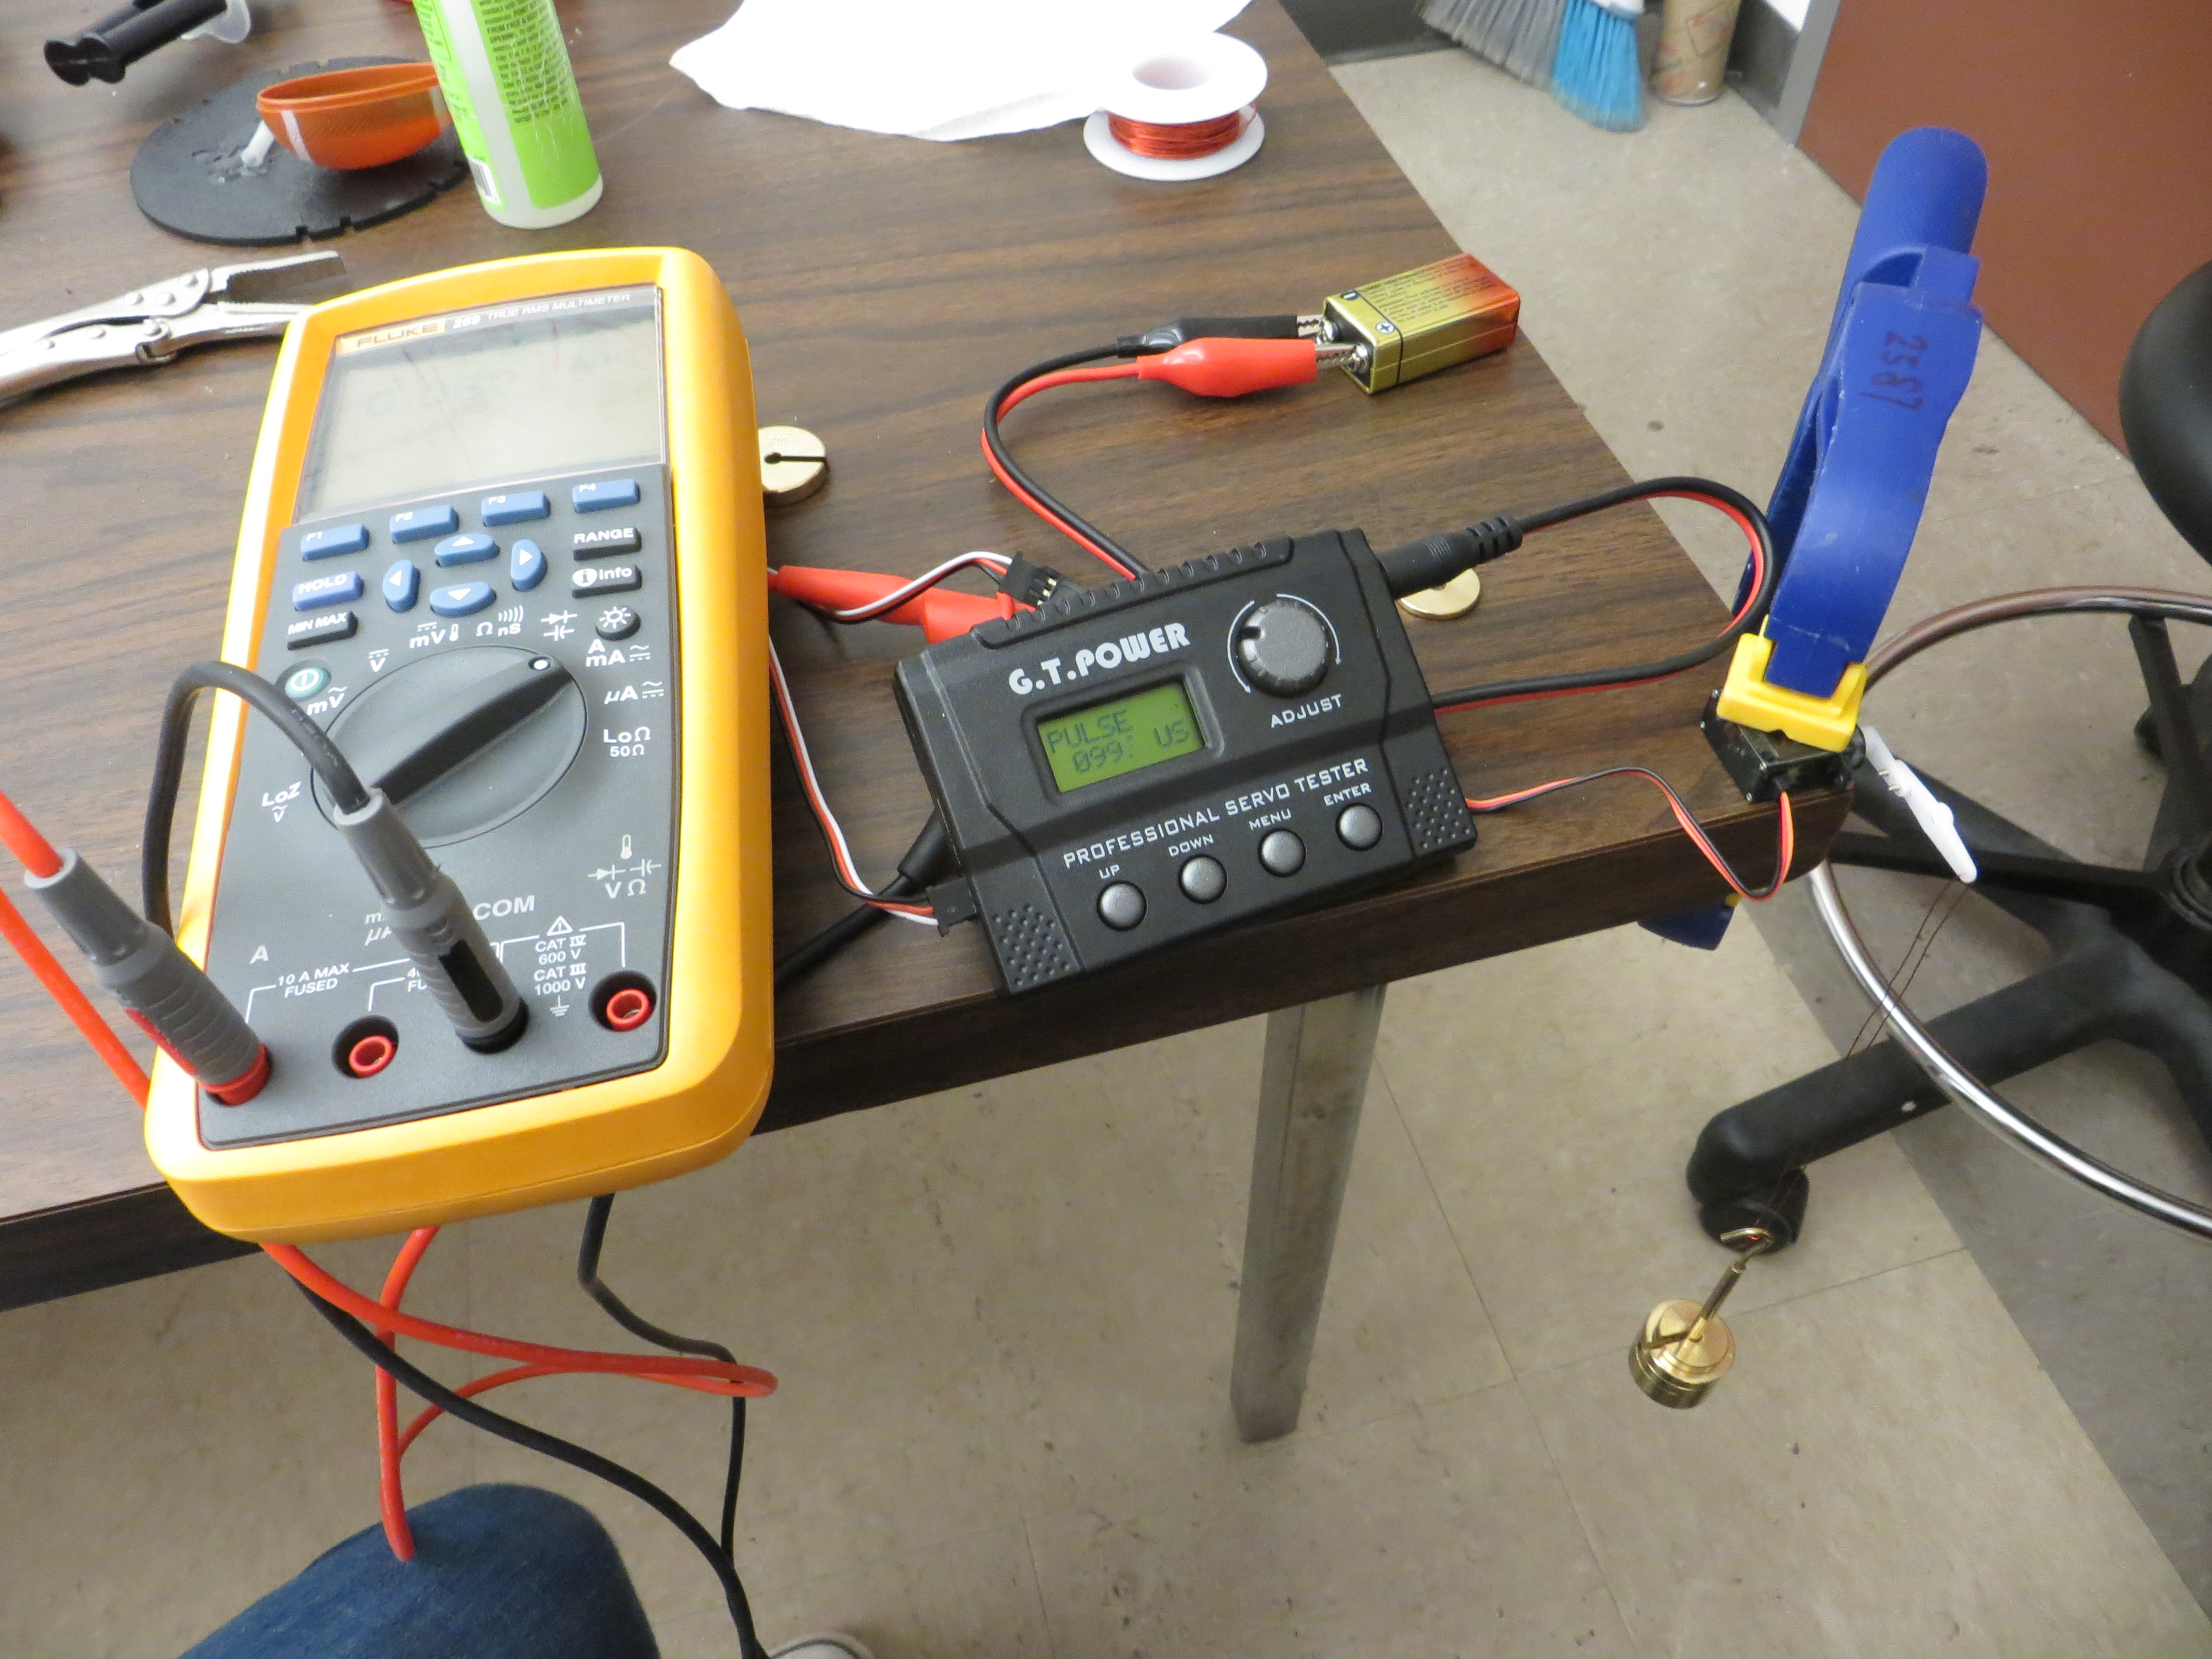
\includegraphics[width=.5\linewidth]{./Figs/full_servotest.jpg}
\end{center}
\caption{Shown are the ammeter, servo controller and servo with a string hanging down in order to properly graph the current vs. force of the lone servo.}
\label{fig:experiment}
\end{figure}

The results of the current-force experiment can be seen below in Figures \ref{fig:BB Test} and \ref{fig:Servo Test}. The measurements we took from both the lone servo and the manipulator servo were strange, because while taking the readings, the Pulse Width Modulation (PWM) Frequency of the servo and the measurement refresh frequency of the ammeter were out of phase, causing the ammeter to read the baseline of the servo, or 0.0050 $\mu$m. These graphs show there is a definite increase in current required for higher forces. 

\begin{figure}[ht]
\begin{minipage}[b]{0.45\linewidth}
\centering
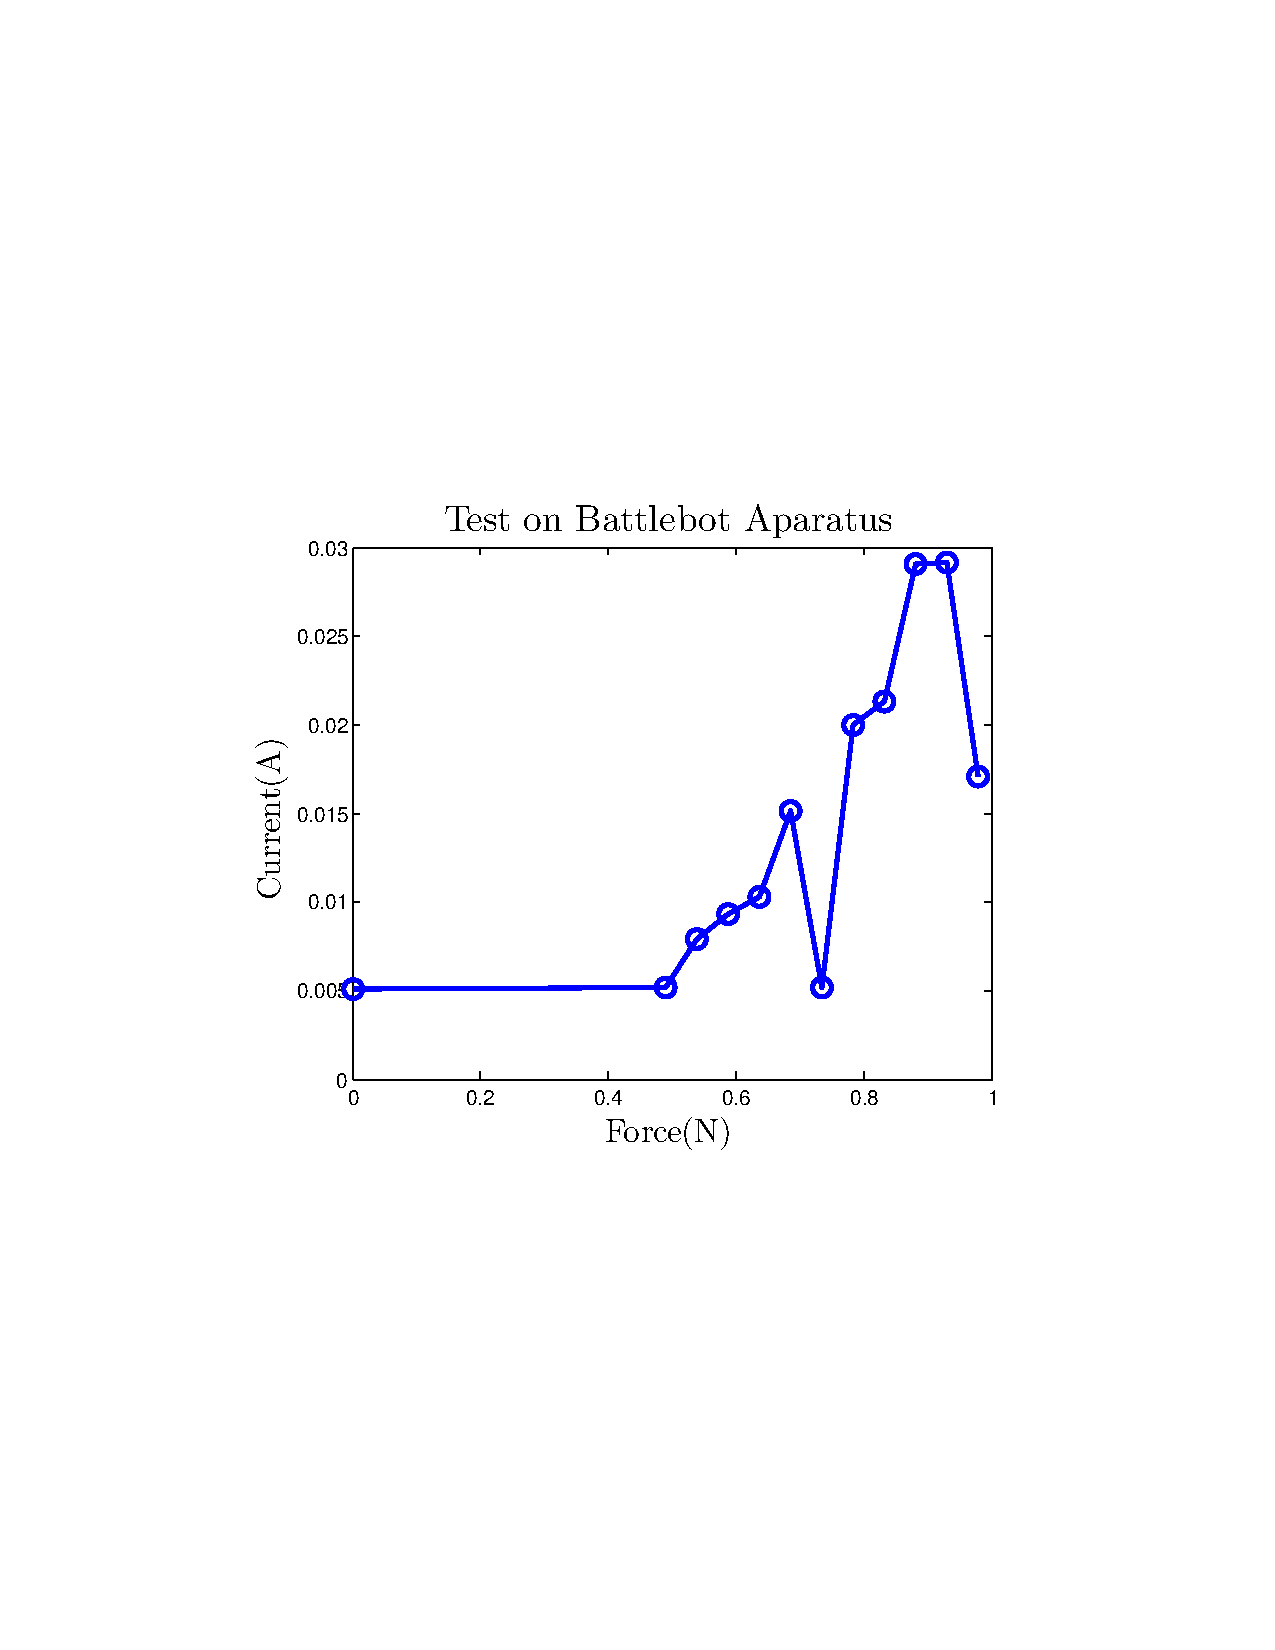
\includegraphics[width=.45\linewidth]{./Figs/Test_on_Battlebot_Aparatus.pdf}
\caption{The graphical result of the Force vs. Current graph of the servo itself.}
\label{fig:BB Test}
\end{minipage}
\hspace{0.5cm}
\begin{minipage}[b]{0.45\linewidth}
\centering
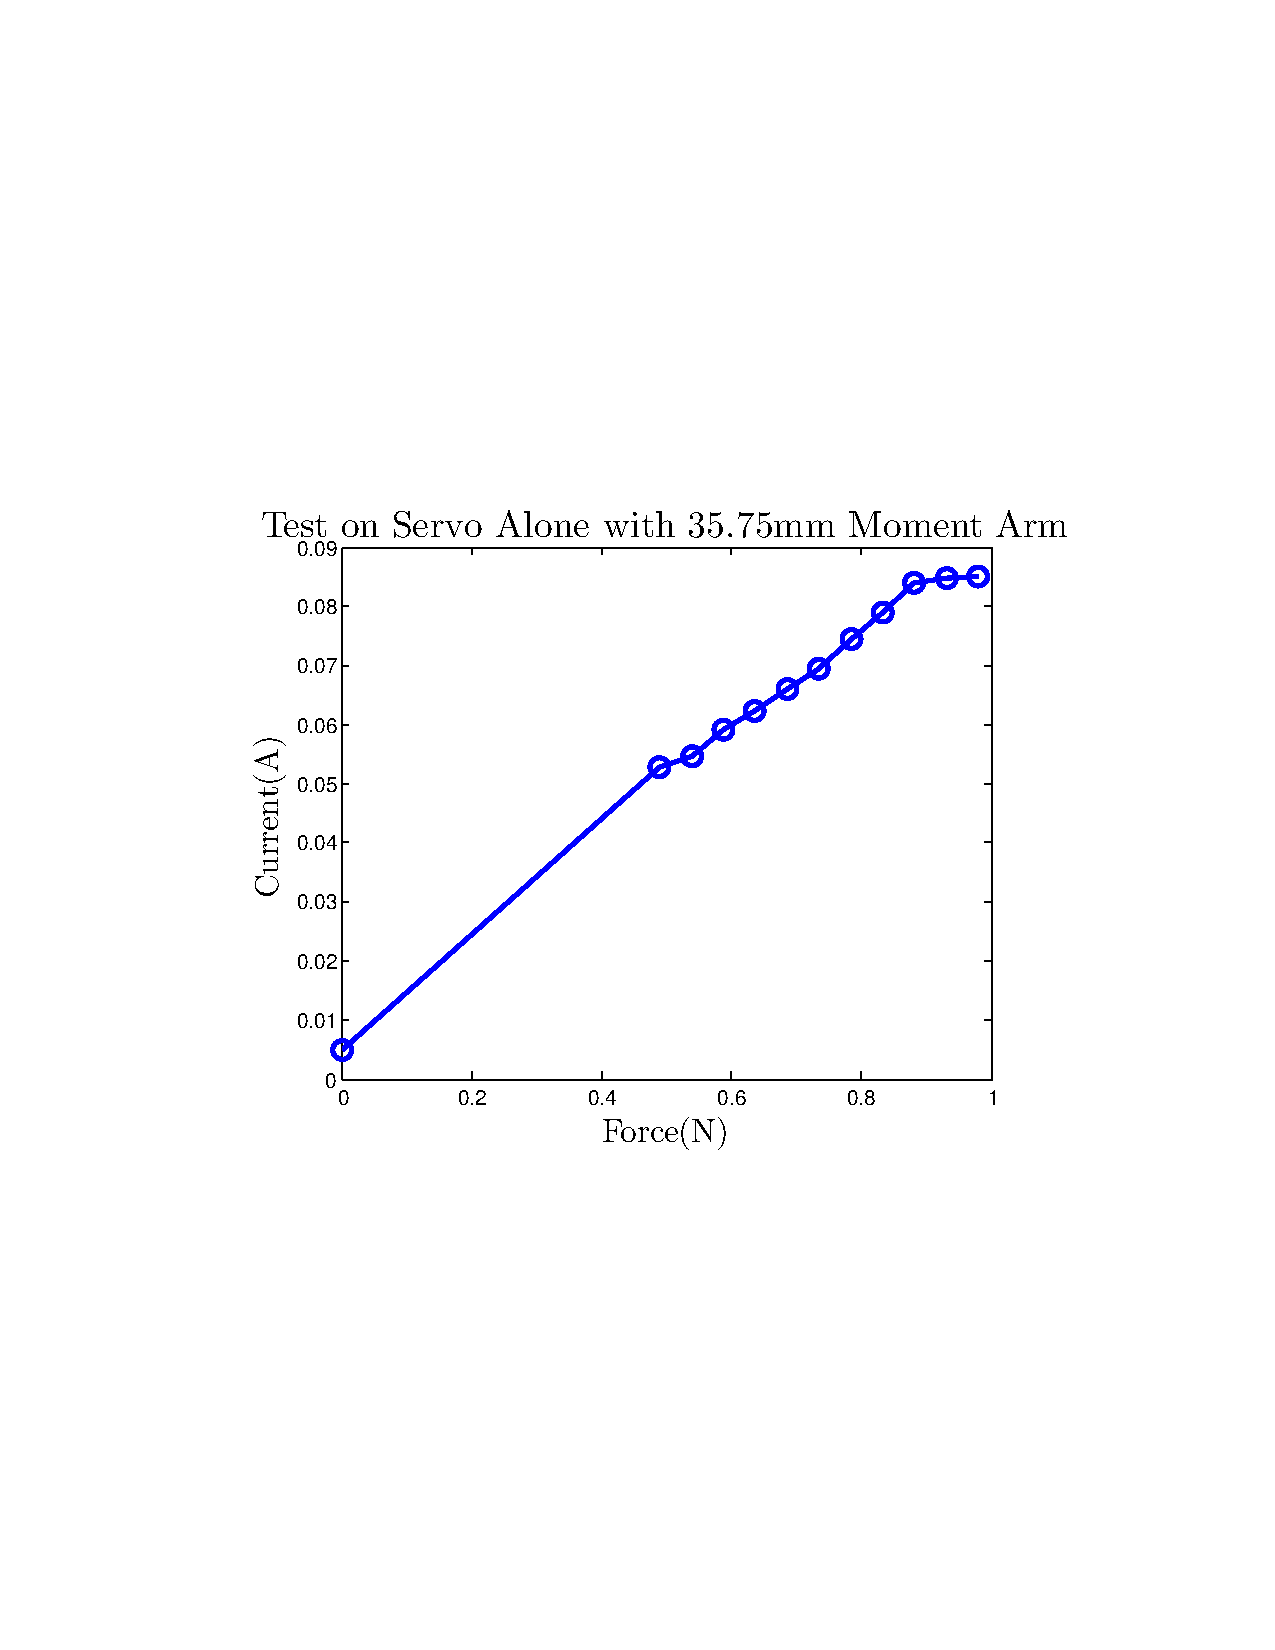
\includegraphics[width=0.45\linewidth]{./Figs/Test_on_servo.pdf}
\caption{The graphical result of the Force vs. Current graph of the servo itself.}
\label{fig:Servo Test}
\end{minipage}
\end{figure}


\end{document}

% % % %
%